% Created 2017-06-16 Fri 09:32
% Intended LaTeX compiler: pdflatex
\documentclass[letterpaper, 9pt, onecolumn, twoside, technote, final]{IEEEtran}
\usepackage[utf8]{inputenc}
\usepackage[T1]{fontenc}
\usepackage{graphicx}
\usepackage{grffile}
\usepackage{longtable}
\usepackage{wrapfig}
\usepackage{rotating}
\usepackage[normalem]{ulem}
\usepackage{amsmath}
\usepackage{textcomp}
\usepackage{amssymb}
\usepackage{capt-of}
\usepackage{hyperref}
\usepackage{color}
\usepackage{listings}
\usepackage{minted}
\usepackage{minted}
\usepackage{makeidx}
\usepackage[lining,tabular]{fbb} % so math uses tabular lining figures
\usepackage[scaled=.95,type1]{cabin} % sans serif in style of Gill Sans
\usepackage[varqu,varl]{zi4}% inconsolata typewriter
\usepackage[T1]{fontenc} % LY1 also works
\usepackage[libertine,bigdelims]{newtxmath}
\usepackage[cal=boondoxo,bb=boondox,frak=boondox]{mathalfa}
\useosf % change normal text to use proportional oldstyle figures
\markboth{Documento de requerimientos para Directed México}%
{Sergio-Feliciano Mendoza-Barrera}
\newcommand{\degC}{$^\circ$C{}}
\author{Sergio-Feliciano Mendoza-Barrera Sergio-Feliciano Mendoza-Barrera}
\date{16/06/2015}
\title{Document Title}
\hypersetup{
 pdfauthor={Sergio-Feliciano Mendoza-Barrera Sergio-Feliciano Mendoza-Barrera},
 pdftitle={Document Title},
 pdfkeywords={R, data science, emacs, ESS, org-mode},
 pdfsubject={Un site nuevo para Directed México},
 pdfcreator={Emacs 26.0.50.1 (Org mode 9.0.8)},
 pdflang={English}}
\begin{document}

\maketitle
\begin{center}
\begin{tabular}{ll}
\textbf{Author} & Sergio-Feliciano Mendoza-Barrera Sergio-Feliciano Mendoza-Barrera\\
\textbf{Email} & sergio@bizland.biz\\
\textbf{Date} & 2017-06-16 09:32:12\\
\end{tabular}
\end{center}
\setcounter{tocdepth}{3}
\tableofcontents

\section{Introduction}
\label{sec:org9344e2c}

\subsection{{\bfseries\sffamily TODO} Abstract}
\label{sec:org863223b}

This document is a demonstration of the \href{https://github.com/thi-ng/org-spec}{thi.ng/org-spec} template,
primarily intended to simplify the creation \& maintenance of technical
specifications written in Org-mode.

All diagrams in this document are autogenerated from embedded code
block snippets in the original \texttt{.org} file. See \hyperref[sec:orgf273336]{Appendix B} for more
information.

Brief outline description of the document\footnote{Example footnote, can also contain \href{https://github.com/thi-ng/org-spec}{links}.}\ldots{}

\subsection{{\bfseries\sffamily DONE} Scope}
\label{sec:orge70993a}

Topics covered by this specification:

\begin{itemize}
\item \hyperref[sec:org5a7642a]{System architecture} - design guidelines, data models, roles \&
responsibilities
\item \hyperref[sec:orge25b676]{Client / server communication} - protocols and implementation details
between system modules
\end{itemize}

\subsection{Status of This Document}
\label{sec:orgdb57c2a}

\textbf{May Be Superseded}

This section describes the status of this document at the time of its
publication. Other documents may supersede this document.

\textbf{Changes since the last version}

\subsection{Conventions}
\label{sec:orgb17798b}

The key words \textbf{MUST}, \textbf{MUST NOT}, \textbf{REQUIRED}, \textbf{SHOULD}, \textbf{SHOULD NOT},
\textbf{RECOMMENDED}, \textbf{MAY}, and \textbf{OPTIONAL} in this specification are to be
interpreted as described in \href{https://tools.ietf.org/html/2119}{RFC2119}.

Since a document and project of this nature deals with a large number
of technologies, each with their own set of acronyms, please refer to
the glossary in \hyperref[sec:org101d683]{Appendix A}, which briefly explains some of them.

\subsubsection{Definition of project specific terms}
\label{sec:orge08f817}

In this document:

\begin{description}
\item[{Term A}] is a\ldots{}
\item[{Term B}] is a\ldots{}
\end{description}
\section{System architecture}
\label{sec:org5a7642a}
\begin{verbatim}
VERSION: 1.0
\end{verbatim}

Example of generating a GraphViz visualization:

\begin{center}
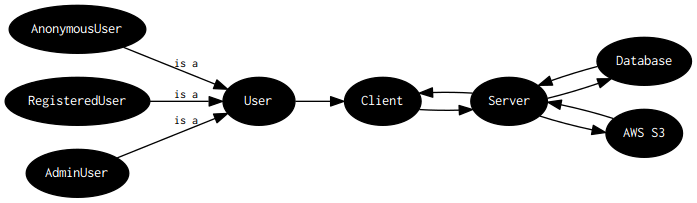
\includegraphics[width=.9\linewidth]{assets/graph.png}
\end{center}

\subsection{System actors, roles \& responsibilities}
\label{sec:orgc7eef90}
\subsubsection{Users}
\label{sec:org69f1a35}
\subsubsection{Client}
\label{sec:org2095bfa}
\subsubsection{Server}
\label{sec:orge531b4b}
\subsection{General system design guidelines}
\label{sec:org9b48fbc}
\subsubsection{User experience}
\label{sec:orgb4b0575}
\subsubsection{Accessibility}
\label{sec:org4b7d82e}
\subsubsection{Data formats}
\label{sec:org3cc81e4}
\subsubsection{Performance}
\label{sec:orgb48e3e1}
\subsubsection{Security}
\label{sec:orgfa8aec1}
\subsubsection{Layered architecture}
\label{sec:org7fffbec}

Example of generating block diagrams from ASCII art using \texttt{ditaa}:

\begin{figure}[htbp]
\centering
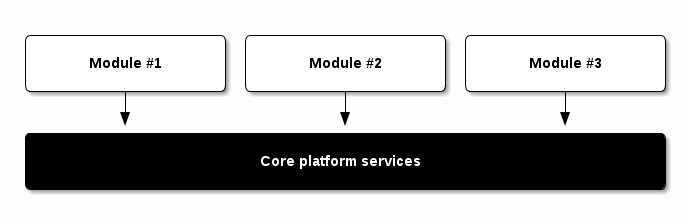
\includegraphics[width=.9\linewidth]{assets/arch.png}
\caption{Top-level, schematic overview of layered client architecture}
\end{figure}

\subsection{Client data model}
\label{sec:orgba050de}
\subsubsection{Overview}
\label{sec:orgf295f55}

Example of generating UML diagrams from textual descriptions using \texttt{plantuml}:

\begin{figure}[htbp]
\centering
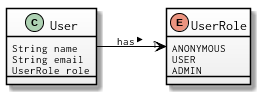
\includegraphics[width=.9\linewidth]{./assets/clientmodel.png}
\caption{Schematic overview of client side data entities}
\end{figure}

In the following sections each data field is expressed with type
information, in Java style pseudo-code form.

\subsubsection{User}
\label{sec:org20dce1a}

\begin{center}
\begin{tabular}{lll}
\textbf{Field} & \textbf{Required} & \textbf{Description}\\
\hline
\texttt{name} & N & User name\\
\texttt{email} & N & User email\\
\texttt{role} & Y & One of possible values defined by \texttt{UserRole}\\
\end{tabular}
\end{center}

Example PlantUML diagram snippet defining the \texttt{User} class in above
diagram. The full diagram itself is defined in the file
\href{https://raw.githubusercontent.com/thi-ng/org-spec/master/sections/diagrams.org}{/sections/diagrams.org}, which is not exported to HTML.

\lstset{language=plantuml,label= ,caption= ,captionpos=b,numbers=none}
\begin{lstlisting}
class User {
  String name
  String email
  UserRole role
}
\end{lstlisting}

\paragraph{User roles}
\label{sec:orgaaad5df}

\begin{center}
\begin{tabular}{ll}
\textbf{Value} & \textbf{Description}\\
\hline
\texttt{ANONYMOUS} & any non-logged in user\\
\texttt{USER} & logged in, registered user with default permissions\\
\texttt{ADMIN} & logged in, registered user with admin permissions\\
\end{tabular}
\end{center}

\lstset{language=plantuml,label= ,caption= ,captionpos=b,numbers=none}
\begin{lstlisting}
enum UserRole {
  ANONYMOUS
  USER
  ADMIN
}
\end{lstlisting}

\subsection{Technologies used}
\label{sec:org1c4b5ec}

This section lists the currently envisaged set of technologies used to
implement the system. Links \& further explanations of the various
projects are provided in \hyperref[sec:org101d683]{Appendix A}.

\begin{description}
\item[{\href{https://github.com/clojure/clojurescript}{ClojureScript}}] Modern dialect of Lisp, compiled to
optimized JavaScript
\end{description}
\section{Client / server communication}
\label{sec:orge25b676}

\subsection{Server API requirements}
\label{sec:orgcc56e11}
\subsubsection{Security considerations}
\label{sec:org8cffd2a}
\subsubsection{HTTP requests}
\label{sec:org2f62342}

The following table summarizes standard HTTP REST requests (as
per \href{https://tools.ietf.org/html/7231}{RFC7231}):

\begin{center}
\begin{tabular}{llll}
\textbf{HTTP Verb} & \textbf{Client intention} & \textbf{HTTP Status} & \textbf{HTTP Status}\\
 &  & (successful) & (error)\\
\hline
\textbf{POST} & create a new resource & 201 \& redirect & 400 / 403 / 404\\
\textbf{PUT} & update an existing resource & 200 / 204 & 400 / 403 / 404 / 409\\
\textbf{GET} & read an existing resource & 200 & 400 / 403 / 404\\
\textbf{DELETE} & delete an existing resource & 200 / 204 & 400 / 403 / 404 / 409\\
\end{tabular}
\end{center}

\subsection{Server routes}
\label{sec:orgfb80a27}
\subsubsection{POST \texttt{/users/login}}
\label{sec:orgace8e51}

\begin{center}
\begin{tabular}{lll}
\textbf{Param} & \textbf{Required} & \textbf{Description}\\
\hline
\texttt{email} & Y & User's registered email address\\
\texttt{pass} & Y & User password\\
\end{tabular}
\end{center}

\textbf{Requires authentication:} NO

\textbf{Description:}
Attempts to authenticate user based on given credentials.

\textbf{Returns:}
\lstset{language=javascript,label= ,caption= ,captionpos=b,numbers=none}
\begin{lstlisting}
{"status": "ok"}
\end{lstlisting}
\lstset{language=javascript,label= ,caption= ,captionpos=b,numbers=none}
\begin{lstlisting}
{"status": "error"}
\end{lstlisting}

\subsection{Clientside SPA routes}
\label{sec:orgd6c1b58}
\subsubsection{Route: \texttt{/login}}
\label{sec:org7a23cb9}

\begin{itemize}
\item Displays login dialog
\item HTTP POST credentials to server \texttt{/login} route
\item Redirects to SPA main page
\end{itemize}

\subsubsection{Route: \texttt{/media/:media\_id}}
\label{sec:orgdf93c4c}

\begin{center}
\begin{tabular}{lll}
\textbf{Param} & \textbf{Type} & \textbf{Description}\\
\hline
\texttt{media\_id} & UUID & Media asset ID\\
\end{tabular}
\end{center}

\begin{itemize}
\item Retrieves media asset from server
\item Displays media asset
\end{itemize}

\section[Appendix A - Glossary]{Appendix A - Glossary\hfill{}\textsc{informative}}
\label{sec:org101d683}
\begin{description}
\item[{AWS}] Amazon Web Services, cloud service provider.
\url{http://aws.amazon.com/}
\item[{ClojureScript}] A modern dialect of Lisp compiling to optimized
JavaScript using Google Closure compiler. \url{https://github.com/clojure/clojurescript}
\item[{CRUD}] Create, Read, Update, Delete - usually refers to
adminstration tasks in CMS / database applications
\item[{EDN}] Extensible Data Notation, lightweight, data exchange format
similar to JSON, but with extensible type support. Native
serialization format for Clojure / ClojureScript.
\url{https://github.com/edn-format/edn}
\item[{Google Closure compiler}] Currently best optimizing JavaScript to
JavaScript compiler. Performs static analysis and whole program
optimizations to allow efficient deployment of large-scale
applications. Supports dynamic module loading.
\url{https://github.com/google/closure-compiler}
\item[{Google Closure library}] Google's standard library for
cross-browser JavaScript application development. All
encompassing \& optimized for Closure compiler.
\url{https://github.com/google/closure-library}
\item[{JSON}] JavaScript Object Notation, lightweight defacto industry
standard data exchange format, especially if parts of a system
involve JavaScript. \url{http://json.org/}
\item[{SPA}] Single-page Application. Refers to a client-side JavaScript
web application model, usually with different UI modules. All
essential assets (HTML, JS, CSS) are loaded only once and lead to
more fluid user experience. Examples: GMail, Google Docs etc.
\item[{Swagger}] Industry defacto standard documentation system for REST
API endpoints. \url{http://swagger.io/}
\item[{UUID}] Universally unique identifier, standardized a 128bit value,
usually expressed as 32 hex characters. \url{https://en.wikipedia.org/wiki/UUID}
\end{description}
\section[Appendix B - Building this document]{Appendix B - Building this document\hfill{}\textsc{informative}}
\label{sec:orgf273336}
This document (including all diagrams) has been generated using the
following tools:

\begin{itemize}
\item \href{https://emacsformacosx.com/}{Emacs}
\item \href{http://orgmode.org}{Org-mode}
\item \href{http://ditaa.sourceforge.net}{Ditaa}
\item \href{http://graphviz.org}{Graphviz}
\item \href{http://plantuml.com/}{PlantUML}
\end{itemize}

\subsection{Re-publish an HTML version}
\label{sec:orge5619fb}

The entire source code for this document is stored in the file
\texttt{index.org}. Please follow these steps to publish an updated HTML
version of the specification:

\begin{enumerate}
\item Install the above listed tools. On OSX \textbf{Ditaa}, \textbf{GraphViz} and
\textbf{PlantUML} can be installed via Homebrew:
\end{enumerate}

\lstset{language=sh,label= ,caption= ,captionpos=b,numbers=none}
\begin{lstlisting}
brew update && brew install ditaa graphviz plantuml
\end{lstlisting}

\begin{enumerate}
\setcounter{enumi}{1}
\item In Emacs type \texttt{M-x load-file RET /path/to/org-theme/config.el}
\item Open the \texttt{index.org} file in Emacs
\item Press \texttt{C-c C-e h o} to launch the export selection dialog, export
as HTML and automatically open the file in your web browser
\end{enumerate}

\textbf{Note}: The export process will re-generate the changelog (only in the
exported HTML), re-create any diagrams and replace any existing
rendered diagram files.

\subsection{Re-publish PDF}
\label{sec:org2b679b6}

Follow the same instructions as for HTML and then print the document
to a PDF file via your browser's print dialog. Print style sheets are
included in the file \texttt{css/styles.css}.
\end{document}
